\section{ARMAX process}

We aim to construct an ARMA process with an additional noise component affecting the output variable. 
The general structure of the model employed for this purpose is illustrated in the diagram below:
\begin{figure}[H]
    \centering
    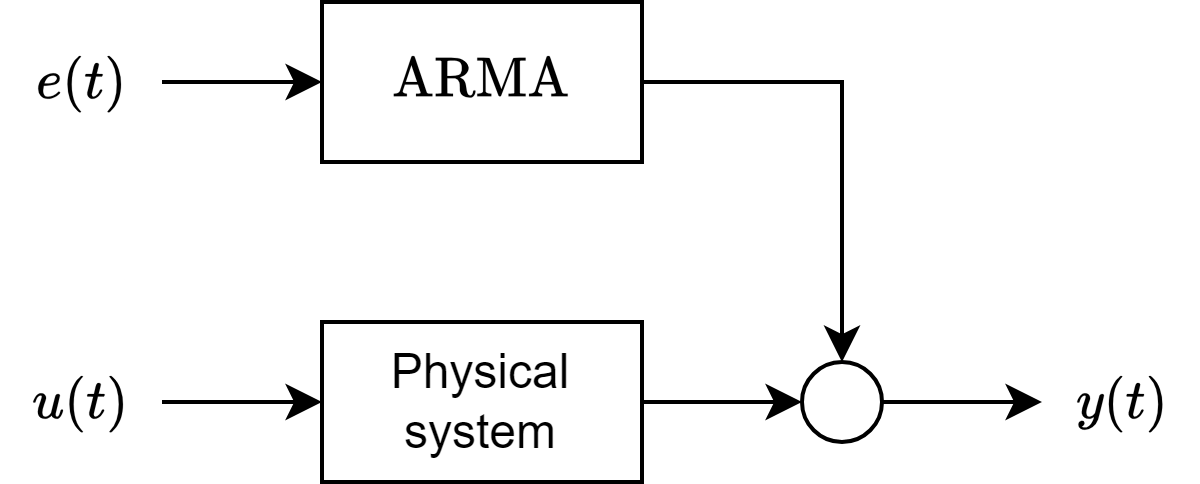
\includegraphics[width=0.5\linewidth]{images/armax.png}
    \caption{ARMAX model}
\end{figure}
The general formulation of this process is expressed as:
\[y(t)=a_1y(t-1)+\cdots+a_m y(t-m)+c_0e(t)+\cdots+c_n e(t-n)+b_0u(t-k)+\cdots+b_p u(t-k-p)\] 
Here, $e(t)\sim WN(\mu,\lambda^2)$
This model comprises three main components: an AutoRegressive process of order $m$, a Moving Average process of order $n$, and an exogenous part denoted as $X_{(k,p)}$.

Within the exogenous part, $p$ indicates the order of the process, signifying the number of past values utilized, while $k$ signifies the pure input-output delay. 
This delay accounts for situations where the influence of $u(t)$ on $y(t)$ is not immediate, typically set to one.

\subsection{Operatorial representation}
Given an ARMAX($m,n,p,k$) model:
\[y(t)=a_1y(t-1)+\cdots+a_m y(t-m)+c_0e(t)+\cdots+c_n e(t-n)+b_0u(t-k)+\cdots+b_p u(t-k-p)\] 
where $e(t)\sim WN(\mu,\lambda^2)$, the model can be expressed in operatorial representation as:
\[y(t)=a_1z^{-1}y(t)+\cdots+a_m z^{-m}y(t)+c_0e(t)+\cdots+c_n z^{-n}e(t)+b_0uz^{-k}(t)+\cdots+b_p z^{-k-p}u(t)\]
By grouping common terms, we obtain:
\[\underbrace{\left(1-a_1z^{-1}-\cdots-a_m z^{-m}\right)}_{A(z)} y(t)=\underbrace{\left(c_0+\cdots+c_n z^{-n}\right)}_{C(z)} e(t)+\underbrace{\left(b_0+\cdots+b_p z^{-p}\right)}_{B(z)} z^{-k}u(t)\]
This can be compactly rewritten as:
\[y(t)=\dfrac{B(z)}{A(z)}z^{-k}u(t)+\dfrac{C(z)}{A(z)}e(t)\]
\begin{figure}[H]
    \centering
    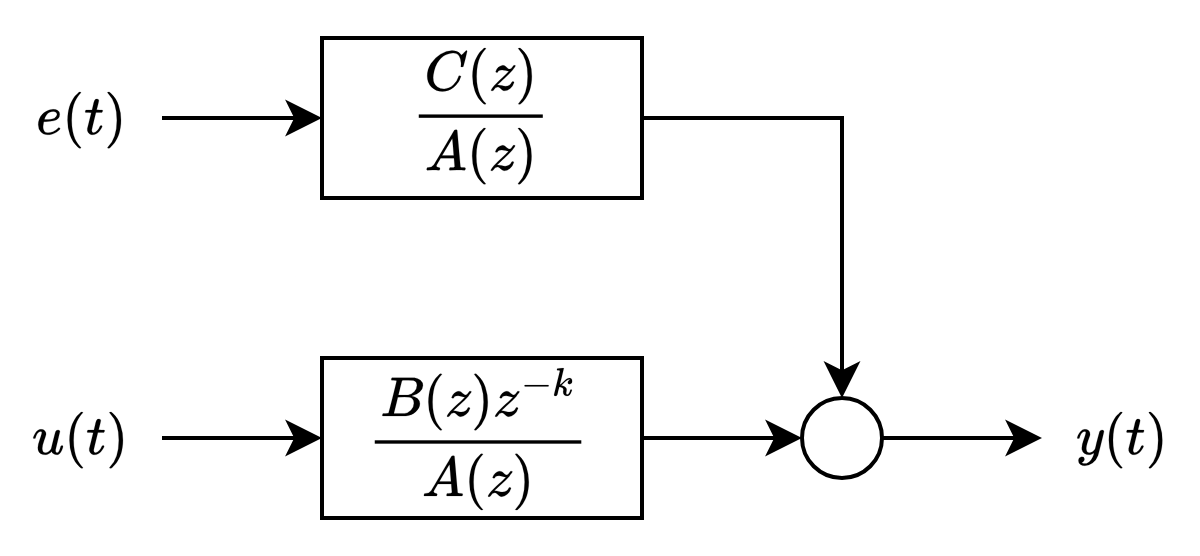
\includegraphics[width=0.5\linewidth]{images/armaxblock.png}
    \caption{ARMAX model in operatorial representation}
\end{figure}
While it's possible to express the transfer functions with both forward and backward shift operators, it's advisable to maintain consistency by using only one type of shift operator within a formula.